\documentclass[12pt,a4paper]{article}
\usepackage{fancyheadings}
\usepackage{pstricks,pst-node,pst-tree}
\usepackage{amsmath}
\usepackage[ansinew]{inputenc}
\usepackage[dvips]{graphicx}
\usepackage[frenchb]{babel}

\title{TP4 {\sc Maple} : Suites et s�ries de fonctions}
\author{}
\date{}


\setlength{\oddsidemargin}{0cm}
\addtolength{\textwidth}{70pt}
\setlength{\topmargin}{0cm}
\addtolength{\textheight}{2cm}
\setlength{\parindent}{0cm}


\pagestyle{fancy}
\lhead{TP4 {\sc Maple}}
\rhead{Suites et s�ries de fonctions}

\newcommand{\R}{\mathbf{R}}
\newcommand{\Z}{\mathbf{Z}}
\newcommand{\C}{\mathbf{C}}
\newcommand{\N}{\mathbf{N}}
 
\newcounter{numsubquestion}
\newcounter{numquestion}
\setcounter{numquestion}{1}
\newenvironment{question}{\setcounter{numsubquestion}{1}\noindent{\bf Exercice \thenumquestion.}}%
{\stepcounter{numquestion}\medskip}

\newenvironment{subquestion}{\smallskip\noindent{\bf \thenumquestion.\thenumsubquestion}}%
{\stepcounter{numsubquestion}\smallskip}

\begin{document}

\maketitle

\begin{question} {\bf Suites de fonctions}\\
On consid�re les trois suites de fonctions suivantes~:
$$\begin{array}{rclr}
  f_n(x) & = & x^n & \quad x\in [0,1]\quad n\in\N \\
  g_n(x) & = & nxe^{-nx} & \quad x\in [0,1]\quad n\in\N \\
  h_n(x) & = & \left(1+\frac{x}{n}\right)^n &\quad x\in\R\quad n\in\N^*  
\end{array}$$

Etudier la convergence (simple, uniforme, uniforme sur certains
compacts) de chacune de ces suites en visualisant leur comportement. 

Commandes {\sc Maple} : {\tt animate} (package {\tt plots}), {\tt limit}.
\end{question}

\begin{question} {\bf Initiation aux s�ries de Fourier}\\
\begin{subquestion}
A l'aide des fonctions {\sc Maple} {\tt floor}, {\tt tan}, {\tt
  arctan}, {\tt cos} et {\tt arccos} d�finir les fonctions
  $2\pi$-p�riodique a l'allure suivante~:
\begin{center}
  \includegraphics[angle=270,width=5.2cm]{TP4007.eps}
  \includegraphics[angle=270,width=5.2cm]{TP4008.eps}
  \includegraphics[angle=270,width=5.2cm]{TP4009.eps}
\end{center}

Commandes {\sc Maple} : option {\tt discont=true} dans la commande
{\tt plot}.
\end{subquestion}

\begin{subquestion}
  Soit $f$ une fonction $2\pi$-p�riodique continue par morceaux sur
  $[0,2\pi]$, on appelle {\it coefficients de Fourier r�els} de $f$
  les suites $\left(a_n\right)_{n\in\N}$ et
  $\left(b_n\right)_{n\in\N}$ d�finies par~:
  \begin{eqnarray*}
    a_n &=& \frac{1}{\pi}\int_{-\pi}^{\pi} f(t) \cos(nt) dt \quad \forall
    n\in\N  \\
    b_n &=& \frac{1}{\pi}\int_{-\pi}^{\pi} f(t) \sin(nt) dt \quad \forall
    n\in\N  
  \end{eqnarray*}
On appelle {\it coefficients de Fourier complexes} de $f$
  la suite $\left(c_n\right)_{n\in\Z}$ d�finie par~:
  \begin{eqnarray*}
    c_n &=& \frac{1}{2\pi}\int_{-\pi}^{\pi} f(t) e^{-i nt} dt \quad\forall
    n\in\Z 
  \end{eqnarray*}

  D�finir les fonctions {\tt c(f,n)}, {\tt a(f,n)} et {\tt b(f,n)} qui
  calculent les coefficients de ces suites pour une fonction $f$
  donn�e. Tester ces fonctions sur les exemples suivants~:
  \begin{eqnarray*}
    x &\mapsto& 2 \\
    x &\mapsto& e^{i3x} \\
    x &\mapsto& (\cos x)^3 \\
    x &\mapsto& (\sin x)^5
  \end{eqnarray*}
Commandes {\sc Maple} : {\tt combine(...,trig)}.  
\end{subquestion}

\begin{subquestion}
On d�finit {\it la s�rie de fourier} de $f$ comme la limite (si elle
existe) de
\begin{eqnarray*}
S_n(f)(x) = \frac{a_0}{2}+\sum_{k=1}^n a_k \cos(kx)+b_k\sin(kx) 
          = \sum_{k=-n}^n c_k e^{ikx}\quad \forall x\in [0,2\pi]    
\end{eqnarray*}
quand $n\to +\infty$.

D�finir les fonctions {\tt FourierR(f,n)} et {\tt FourierC(f,n)}
qui calculent les sommes partielles pr�c�dentes avec les coefficients
r�els pour {\tt FourierR} et avec les coefficients complexes pour {\tt
  Fourierc}. Tester ces fonctions. Il est d�conseill� d'utiliser {\tt sum}.
\end{subquestion}

\begin{subquestion}
   On d�finit {\it la somme de F�jer} de $f$ comme la limite (si elle
   existe) de
$$\sigma_n(f)=\frac{S_0(f)+S_1(f)+\cdots+S_n(f)}{n+1}$$
D�finir les fonctions {\tt FejerR(f,n)} et {\tt FejerC(f,n)} qui
calculent cette somme partielle � partir des fonctions pr�c�dentes. 
\end{subquestion}

\begin{subquestion}
Etudier graphiquement le
comportement des s�ries de Fourier et des sommes de F�jer des trois
fonction de la question {\bf 2.1}. Quel type de convergence obtient-on ?
\end{subquestion}
\end{question}

\begin{question} 
  On d�finit
  $$u_n=\frac{(-1)^{n+1}}{n}\quad n\in\N^*$$
  Comparer � l'aide de {\sc Maple} les limites suivantes
  $$\sum_{n=1}^{+\infty} u_n\text{ et }
    \sum_{n=1}^{+\infty} u_{2n-1}+u_{4n-2}+u_{4n}$$
  Interpr�ter et justifier math�matiquement ces r�sultats.
\end{question}
\end{document}

